\chapter{Diseño de la validación}
\label{ch:validacion}

Este capítulo describe cómo se ha evaluado cada parte del sistema: con qué datos, con qué métricas y qué precauciones se han tomado para que las cifras sean fiables. Los resultados se presentan en el capítulo~\ref{ch:resultados}. Todas las pruebas son reproducibles: cada una tiene un programa en la carpeta \texttt{backend/validacion} del repositorio (tabla~\ref{tab:scripts-validacion}) que genera sus resultados en forma de tablas.

\section{Principios comunes}
\label{s:principios-validacion}

\begin{itemize}
    \item \textbf{Separar los datos de ajuste de los de medida.} Cuando una parte del sistema se ha mejorado mirando sus fallos sobre un conjunto de datos, las cifras sobre ese conjunto dejan de ser una medida limpia. Por ello, siempre que ha sido posible se ha reservado un conjunto de prueba que no se ha usado para tomar decisiones, y se indica expresamente cuándo una cifra procede de datos usados para ajustar.
    \item \textbf{Respuesta correcta independiente del sistema.} La respuesta correcta de cada caso (\gls{ground-truth}) se obtiene del texto de los PDF, se escribe a mano o se anota manualmente, nunca a partir de la salida del propio sistema.
    \item \textbf{Incertidumbre.} Los conjuntos de prueba son pequeños, por lo que cada porcentaje se acompaña de su intervalo de confianza al 95\,\% calculado con el método de Wilson \parencite{wilson1927probable}, más adecuado que la aproximación normal con pocas muestras o proporciones cercanas al 100\,\%.
    \item \textbf{Comparaciones pareadas.} Cuando dos variantes se evalúan sobre los mismos casos (por ejemplo, el asistente con y sin \gls{rag}), la diferencia se contrasta con la prueba exacta de McNemar \parencite{mcnemar1947note}, que solo tiene en cuenta los casos en los que las dos variantes discrepan.
\end{itemize}

\section{Lectura de tickets}
\label{s:val-donut}

\subsection{Conjuntos de datos}
Los 91 tickets del conjunto de datos se usaron para entrenar el modelo (77) o para elegir la mejor época (14), por lo que no sirven para medir cómo se comporta con tickets nuevos. Para obtener una medida limpia se reunieron \textbf{17 tickets nuevos} en PDF, correspondientes a compras posteriores a la creación del conjunto de datos (de mayo a octubre de 2026). Los dos más recientes tienen además una cabecera de columnas distinta, introducida por Mercadona en octubre de 2026. Las cifras se dan por separado para los tickets nuevos, que son la medida principal, y para los 14 de validación.

La respuesta correcta se obtiene automáticamente del texto del PDF con el mismo analizador que generó el conjunto de datos (sección~\ref{s:extraccion-validada}), incluida la comprobación de que la suma de los importes coincide con el total. El modelo, en cambio, recibe la imagen de la página, exactamente igual que en la aplicación.

\subsection{Fotografías simuladas}
\label{s:fotos-simuladas}
No se disponía de fotografías de tickets en papel con su PDF correspondiente, ya que el autor usa el ticket digital. Para estimar cómo se comporta el modelo con fotografías se simularon a partir de la imagen de cada PDF los efectos de una foto hecha con el móvil: el ticket sobre una mesa, girado y en perspectiva, con iluminación desigual, ruido del sensor, desenfoque, menor resolución y compresión JPEG. Se generaron tres niveles de dificultad con semilla fija (tabla~\ref{tab:niveles-foto} y figura~\ref{fig:fotos-simuladas}). Como cada imagen procede de un PDF, la respuesta correcta se sigue obteniendo automáticamente.

\begin{table}[htbp]
    \caption{\label{tab:niveles-foto}Parámetros de las fotografías simuladas}
    \begin{tabularx}{\textwidth}{@{}Xccc@{}}
        \toprule
        \textbf{Efecto} & \textbf{Leve} & \textbf{Media} & \textbf{Fuerte} \\
        \midrule
        Giro máximo & 2$^{\circ}$ & 5$^{\circ}$ & 9$^{\circ}$ \\
        Deformación de perspectiva (proporción del tamaño) & 2\,\% & 5\,\% & 8\,\% \\
        Sombra (oscurecimiento máximo) & 15\,\% & 30\,\% & 45\,\% \\
        Desenfoque gaussiano (radio en píxeles) & 0,6 & 1,1 & 1,7 \\
        Ruido (desviación típica) & 4 & 8 & 12 \\
        Escala de la imagen & 85\,\% & 70\,\% & 55\,\% \\
        Calidad JPEG & 85 & 70 & 55 \\
        \bottomrule
    \end{tabularx}
\end{table}

\begin{figure}[htbp]
    \centering
    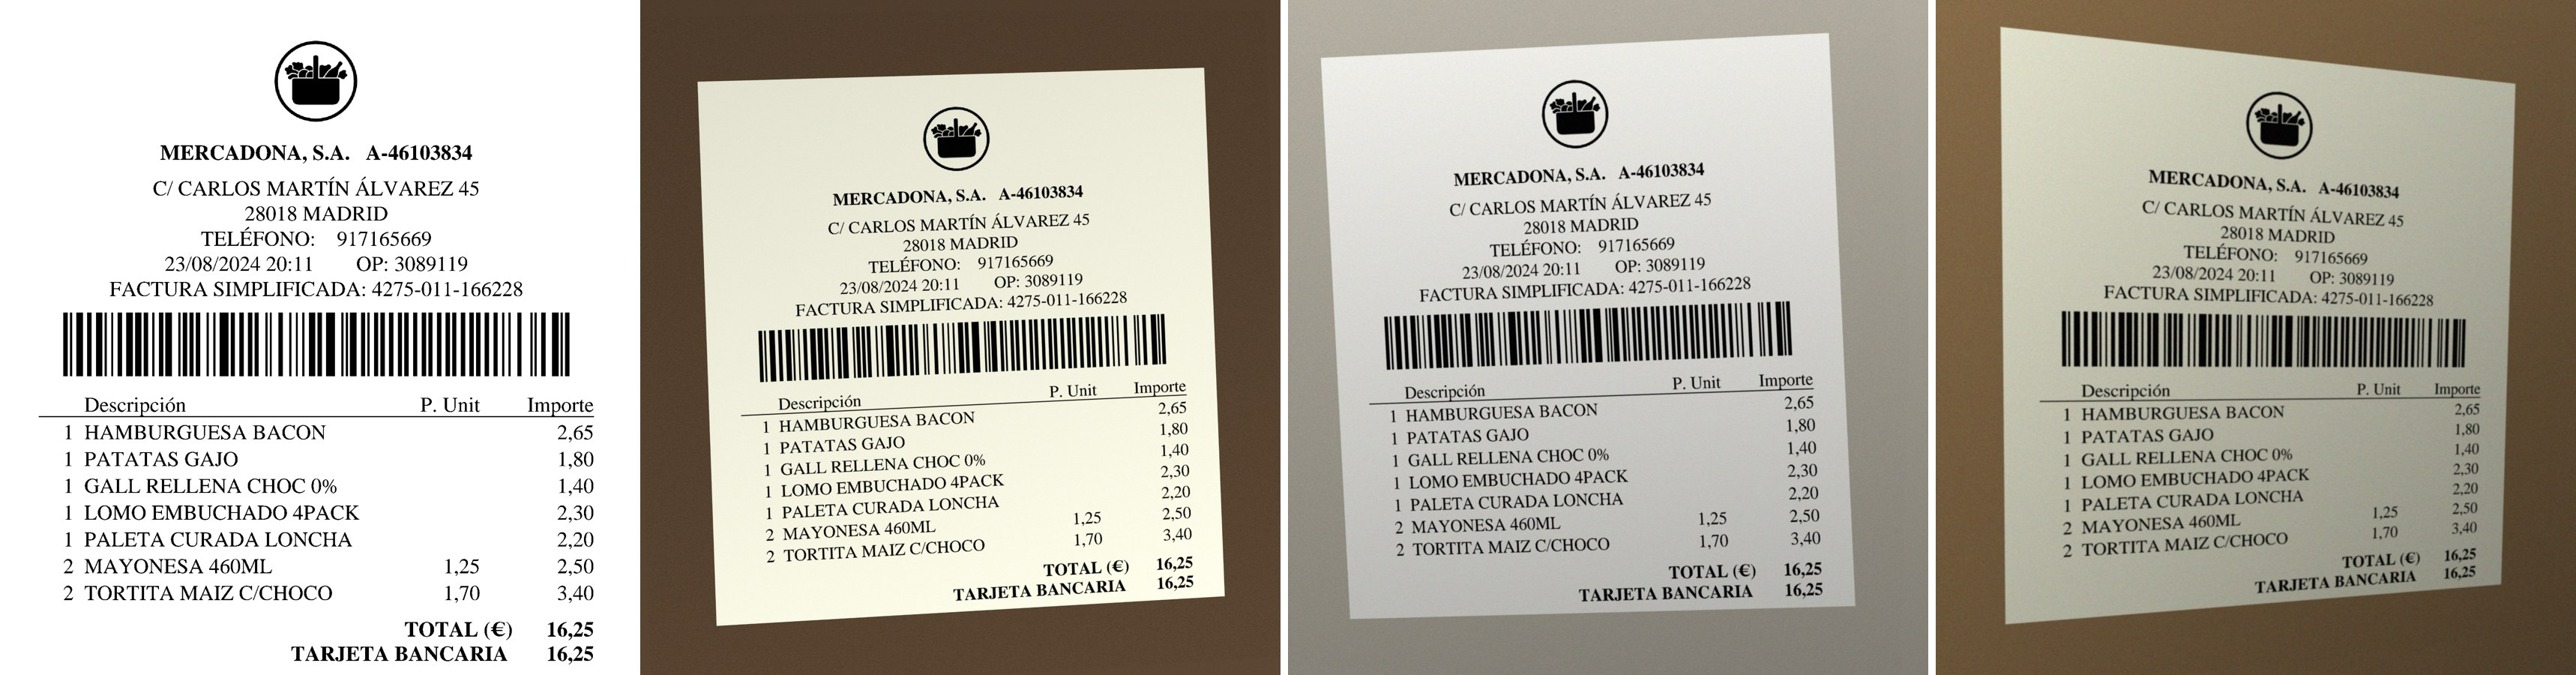
\includegraphics[width=\textwidth]{figuras/fotos_sinteticas.jpg}
    \caption{Parte superior de un ticket de validación: imagen del PDF y fotografías simuladas de nivel leve, medio y fuerte.}
    \label{fig:fotos-simuladas}
\end{figure}

Esta simulación no reproduce el papel térmico arrugado o desvaído, los reflejos ni el texto cortado, por lo que es una prueba de robustez y no sustituye a una evaluación con fotografías reales.

\subsection{Métricas}
A las métricas del entrenamiento (ticket perfecto, ticket casi perfecto, F1 de productos y acierto de la fecha y del total) se añaden:

\begin{itemize}
    \item por línea de producto, el acierto del nombre, de la cantidad y del importe, y la \gls{cer} del nombre, es decir, el número de caracteres que habría que cambiar para llegar al nombre correcto dividido entre su longitud;
    \item el número de líneas no leídas o inventadas y de lecturas cortadas;
    \item la \textbf{detección}: qué proporción de los tickets con algún error manda la aplicación a revisión (porque la suma no cuadra, la fecha es dudosa o la lectura está incompleta) y cuántos tickets correctos manda a revisión sin motivo;
    \item el tiempo de lectura por ticket en el equipo del autor, sin \gls{gpu} dedicada al modelo.
\end{itemize}

Para comparar línea a línea, las líneas leídas se emparejan con las reales siguiendo el orden del ticket y el parecido de los nombres.

\section{Corrector de nombres y revisión de fechas}
\label{s:val-corrector-fechas}

\subsection{Corrector de nombres}
El corrector se evaluó con dos pruebas complementarias:

\begin{enumerate}
    \item \textbf{Errores reales del modelo}: las líneas emparejadas de la prueba anterior (PDF y fotografías simuladas de los tickets nuevos y de validación) en las que el nombre leído no difiere en más de la mitad de sus caracteres del real. El límite descarta los emparejamientos entre productos distintos, frecuentes en las fotografías difíciles.
    \item \textbf{Errores simulados}: a cada nombre de producto de los 91 tickets del conjunto de datos se le introduce un error típico de lectura (una o dos letras parecidas cambiadas, una letra de más o de menos, una palabra partida o dos palabras juntas). Para no hacer trampa, el vocabulario del corrector incluye el catálogo y los nombres de los \emph{otros} tickets, nunca los del ticket evaluado. También se pasan los nombres sin error, para medir con qué frecuencia el corrector estropea un nombre correcto.
\end{enumerate}

Se consideran tres situaciones: un usuario con historial (catálogo y tickets anteriores), un usuario nuevo (solo el catálogo) y la subida de un PDF, en la que se dispone además de los nombres exactos del texto del documento. Cada nombre se clasifica según si estaba bien o mal leído y según lo que hace el corrector: no tocarlo, corregirlo bien, corregirlo solo en parte (queda más cerca del real), corregirlo mal o proponer una sugerencia.

\subsection{Revisión de fechas}
Las fotografías simuladas no tienen metadatos EXIF, de modo que la fecha de referencia se simula en varios escenarios: foto hecha el mismo día de la compra, foto hecha entre uno y tres días después, foto sin ninguna referencia y PDF descargado entre 0 y 120 días después. Se evalúan dos conjuntos:

\begin{enumerate}
    \item las \textbf{fechas leídas por el modelo} en la prueba de lectura (93 lecturas de fotografías simuladas y 31 de PDF);
    \item \textbf{errores simulados} sobre las fechas de los 108 tickets disponibles, cinco por fecha, de los tipos observados en las lecturas reales: dígitos parecidos, día y mes intercambiados, dígitos del día o del mes intercambiados, año equivocado y mes leído como \enquote{09}, el error más frecuente en las fotografías.
\end{enumerate}

Para cada fecha se mide si la aplicación avisa y si la fecha que propone es la real. Las fechas bien leídas se usan para medir las falsas alarmas. La búsqueda de la fecha por parecido de dígitos (sección~\ref{s:revision-fecha}) se añadió después de observar los errores del primer conjunto, por lo que su resultado sobre ese conjunto es optimista; el segundo es la medida más neutral.

\section{Detección de tickets repetidos}
\label{s:val-repetidos}
Se usan los 108 tickets distintos disponibles en PDF (los 91 del conjunto de datos y los 17 nuevos) y las lecturas del modelo obtenidas en la prueba de lectura. Se miden dos tipos de error, opuestos entre sí:

\begin{itemize}
    \item \textbf{Falsos positivos}: que el sistema tome dos compras \emph{distintas} por la misma, lo que impediría al usuario guardar un ticket real. Se cuentan los pares de tickets distintos que comparten la huella de contenido, el número de factura o la fecha y el total.
    \item \textbf{Repetidos no detectados}: que el usuario vuelva a subir una compra que ya tiene guardada y el sistema no se dé cuenta, con lo que el gasto se contaría dos veces.
\end{itemize}

Si se sube exactamente el mismo archivo, el repetido se detecta siempre por su \textit{hash}, por lo que la prueba se centra en el caso difícil: la misma compra llega en un archivo \emph{distinto}, ya sea otro PDF del mismo ticket (31 lecturas) o una fotografía del ticket en papel (93 lecturas de las fotografías simuladas). Se supone que el ticket ya guardado es correcto, porque el usuario lo revisó al guardarlo, mientras que el nuevo lo lee el modelo y puede contener errores. En un PDF esto no es un problema, porque el número de factura se extrae del texto del documento y no depende de la lectura del modelo. En una fotografía, en cambio, no hay número de factura, y si el modelo lee mal la fecha o el total no hay forma de relacionarla con el ticket guardado. Se mide, por tanto, en el peor caso: el usuario no corrige nada en la pantalla de revisión. Si corrige la fecha y el total antes de guardar, la comprobación que se repite al guardar detecta el repetido con los datos ya corregidos.

Conviene precisar que esta prueba se hace sobre fotografías simuladas y no es un registro del uso real de la aplicación, en el que la mayoría de los tickets se suben en PDF.

Como comprobación adicional, se generaron seis extractos bancarios simulados con formatos distintos para verificar que se rechazan sin pasar por el modelo, mientras que todos los tickets se aceptan.

\section{Categorización de productos}
\label{s:val-clustering}

\subsection{Etiquetas de referencia}
Las categorías guardadas en los tickets las había asignado el propio buscador del catálogo, por lo que usarlas como respuesta correcta daría a este un 100\,\% de acierto por construcción. Para evitarlo, se revisaron las categorías de los 280 productos distintos de los tickets, consultando el catálogo y el significado de las abreviaturas. La revisión se hizo con ayuda de una herramienta de \gls{ia} y el autor comprobó una muestra de 52 productos: coincidió en todos los casos comparables. Se corrigieron 28 productos mal clasificados por el buscador (por ejemplo, unas bolas de cereales con chocolate clasificadas como queso).

\subsection{Experimento}
Para asignar automáticamente una categoría a un producto como \texttt{LECHE SEMI DESN} hay que tomar dos decisiones: cómo convertir su nombre en algo que el ordenador pueda comparar con otros nombres (la \emph{representación}) y cómo decidir la categoría a partir de esa comparación (el \emph{método de clasificación}). El experimento prueba varias opciones de cada una y las combina entre sí. Todos los métodos se implementaron con scikit-learn \parencite{pedregosa2011scikit}.

Las representaciones comparadas son:

\begin{itemize}
    \item \textbf{Por fragmentos de letras} (TF-IDF de caracteres): dos nombres se parecen si comparten muchos trozos de letras, como \texttt{LECH SEMI} y \textit{leche semidesnatada}. Es la opción natural para las abreviaturas de los tickets.
    \item \textbf{Por palabras completas} (TF-IDF de palabras) y una \textbf{combinación de letras y palabras}, comprimida a 256 valores.
    \item \textbf{Por significado} (\textit{embeddings} de los modelos bge-m3 y nomic-embed-text): un modelo de lenguaje sitúa cerca nombres de significado parecido aunque no compartan letras, como \textit{yogur} y \textit{postre lácteo}.
    \item \textbf{Significado y letras a la vez}, uniendo las dos representaciones anteriores.
\end{itemize}

Los métodos de clasificación comparados son los de la sección~\ref{s:clasificador-hibrido}:

\begin{itemize}
    \item \textbf{Clustering}: se forman grupos de productos parecidos y cada grupo toma la categoría más frecuente entre sus productos conocidos; un producto nuevo recibe la categoría del grupo al que más se parece. Se probó K-Means con 26 grupos (uno por categoría), 148 (aproximadamente uno por subcategoría) y 444 (grupos más pequeños); el clustering jerárquico de Ward, que construye los grupos uniendo poco a poco los productos más parecidos, con 148 y 444 grupos; y HDBSCAN, que decide por sí mismo cuántos grupos hay, exigiendo al menos tres productos por grupo.
    \item \textbf{Métodos de referencia}, para saber si el clustering aporta algo: el \textbf{vecino más cercano} (1-NN), que copia la categoría del producto conocido más parecido; los \textbf{cinco vecinos más cercanos}, que votan entre ellos; y el \textbf{buscador del catálogo} que ya usaba la aplicación.
\end{itemize}

Cada combinación se evalúa en tres escenarios, de menos a más parecidos al uso real de la aplicación:

\begin{enumerate}
    \item[A.] \textbf{Solo catálogo}: se clasifican productos del catálogo aprendiendo del resto del catálogo. Es el caso fácil, porque los nombres están completos y las categorías son las oficiales.
    \item[B.] \textbf{Del catálogo a los tickets}: se aprende solo del catálogo y se clasifican los 280 productos de los tickets, con sus nombres abreviados. Equivale a un usuario nuevo que todavía no tiene tickets guardados.
    \item[C.] \textbf{Tickets con historial}: se clasifican los productos de los tickets aprendiendo del catálogo y de los demás tickets. Es la situación real de la aplicación, que aprovecha los tickets que el usuario ya ha guardado.
\end{enumerate}

En los escenarios A y C los productos se dividen en cinco partes y cada parte se clasifica aprendiendo de las otras cuatro (validación cruzada de cinco particiones). Así ningún producto se clasifica teniendo ya su propia respuesta entre los datos de aprendizaje.

En todos los casos se mide el porcentaje de productos con la categoría y la subcategoría correctas. Además, para saber si los grupos que forma el clustering por sí solo se parecen a las categorías de Mercadona, se calculan dos medidas de coincidencia entre grupos y categorías, el índice de Rand ajustado (ARI) \parencite{hubert1985comparing} y la información mutua normalizada, que valen 0 si los grupos no tienen nada que ver con las categorías y 1 si coinciden exactamente; y el coeficiente de silueta \parencite{rousseeuw1987silhouettes}, que indica si los grupos están bien separados entre sí. Por último, en el escenario C se prueba la combinación final del sistema: se usa el buscador cuando está suficientemente seguro y, si no, el vecino más cercano o el clustering. Para elegir a partir de qué confianza fiarse del buscador se prueban cinco umbrales entre 0,55 y 0,95.

\section{Asistente de consulta de gastos}
\label{s:val-chat}

\subsection{Bancos de preguntas}
Se escribieron a mano dos bancos de preguntas, cada una con la consulta correcta que debería generarse:

\begin{itemize}
    \item \textbf{Banco de desarrollo} (116 preguntas): básicas (20), coloquiales (20), combinadas (20), con filtros (20), con periodos (15), de continuación de una pregunta anterior (10) y fuera de ámbito o saludos (7), más 4 casos límite que el motor no cubría al empezar y que se analizan aparte. Se usó para analizar los fallos y mejorar el sistema.
    \item \textbf{Banco de prueba} (40 preguntas nuevas de los mismos tipos), reservado para las cifras finales.
\end{itemize}

Ninguna pregunta coincide con los ejemplos de las instrucciones del modelo de lenguaje ni con las frases del clasificador de intenciones, lo que se comprobó automáticamente. Todas se evalúan sobre una copia fija de los 91 tickets del autor y con una fecha de referencia fija (20 de abril de 2026), para que expresiones como \enquote{el mes pasado} tengan siempre la misma respuesta.

\subsection{Métricas}
Una pregunta puede traducirse correctamente a consultas distintas que dan el mismo resultado (por ejemplo, con o sin un filtro que no cambia nada). Por eso la métrica principal no compara las consultas, sino sus \textbf{resultados}: se ejecutan la consulta generada y la correcta y se considera acierto si dan el mismo número, el mismo primer elemento (o los mismos $k$ primeros si la pregunta pide $k$), el mismo conjunto o la misma serie temporal. Además se miden la coincidencia exacta de la consulta campo a campo y el tiempo de respuesta. El evaluador se verificó sustituyendo el modelo por uno simulado que devuelve siempre la consulta correcta, con el que se obtiene el 100\,\% de acierto.

\subsection{Evaluación del RAG}
\label{s:val-rag}
El \gls{rag} se evaluó de dos formas:

\begin{enumerate}
    \item \textbf{Sobre los bancos}: con la base de ejemplos formada por el banco de desarrollo. Al evaluar el propio banco de desarrollo se excluye la pregunta evaluada de los ejemplos recuperables (validación dejando uno fuera).
    \item \textbf{Experimento de adaptación}, para medir el escenario para el que está pensado: que el asistente aprenda de las respuestas que el usuario valida. Se escribieron 20 preguntas \enquote{semilla} con su consulta correcta, con expresiones que no aparecen ni en las instrucciones ni en los bancos (\enquote{mi compra gorda}, \enquote{50 pavos}, \enquote{lo que más echo al carro}). Otra herramienta de \gls{ia}, distinta de la usada para escribir las semillas, redactó dos formas diferentes de hacer cada pregunta, con la instrucción de cambiar el vocabulario y mantener el significado. Se revisaron sin ejecutar el sistema y se descartaron tres que cambiaban el significado, eran ambiguas o casi copiaban la semilla, quedando 37 preguntas. Se comparan tres condiciones: el modelo sin \gls{rag}, con \gls{rag} sobre el banco de desarrollo y con \gls{rag} sobre el banco de desarrollo más las semillas, que simulan respuestas valoradas positivamente por el usuario.
\end{enumerate}

\section{Programas de validación}
La tabla~\ref{tab:scripts-validacion} resume los programas que implementan las pruebas.

\begin{table}[htbp]
    \caption{\label{tab:scripts-validacion}Programas de validación (carpeta \texttt{backend/validacion})}
    \begin{tabularx}{\textwidth}{@{}lX@{}}
        \toprule
        \textbf{Programa} & \textbf{Prueba} \\
        \midrule
        \texttt{evaluar\_donut.py} & Lectura de tickets en PDF y en fotografías \\
        \texttt{generar\_fotos\_sinteticas.py} & Fotografías simuladas en tres niveles \\
        \texttt{evaluar\_corrector.py} & Corrector de nombres (errores reales y simulados) \\
        \texttt{evaluar\_fechas.py} & Revisión de fechas (fechas reales y errores simulados) \\
        \texttt{evaluar\_documentos.py} & Tickets repetidos y rechazo de documentos que no son tickets \\
        \texttt{evaluar\_clustering.py} & Representaciones, clustering y vecinos más cercanos \\
        \texttt{evaluar\_hibrido.py} & Combinación del buscador con el vecino más cercano o el clustering \\
        \texttt{generar\_banco.py} & Bancos de preguntas de desarrollo y prueba \\
        \texttt{evaluar\_chat.py} & Asistente con reglas, con modelo de lenguaje y con \gls{rag} \\
        \texttt{generar\_semillas\_rag.py} & Semillas y paráfrasis del experimento de adaptación \\
        \bottomrule
    \end{tabularx}
\end{table}
